\subsection{Peak Traffic Demand}\label{subsec:peakratio}

\begin{figure}[ht!]
%\hspace*{-0.2in}
\begin{minipage}{0.90\linewidth}
\centering
\begin{subfigure}[b]{0.90\linewidth}
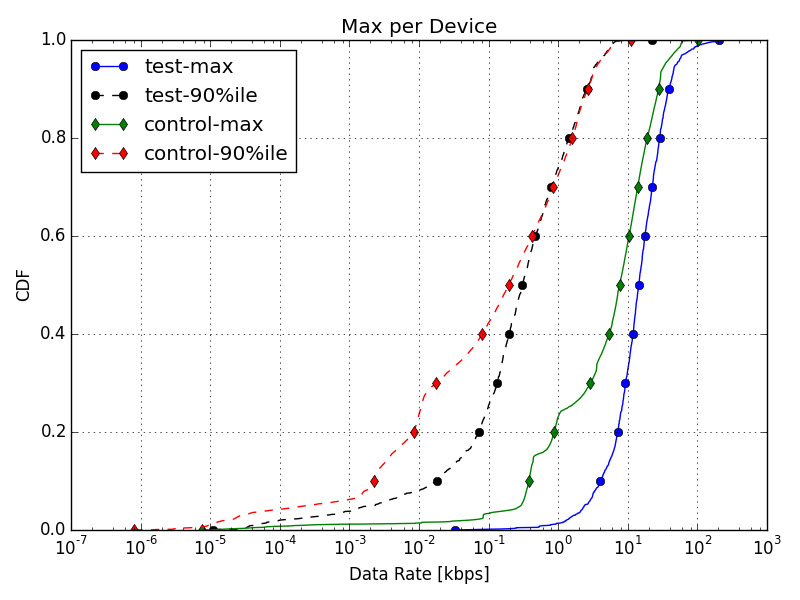
\includegraphics[width=\linewidth]{figures/cdf-max-per-device.png}
  \caption{CDF of max per device: test set has higher (max) average data rate 
below 10 kbps.  30\% of devices in the control set have a max data rate of 2 
kbps while 30\% of test set has a max data rate of 10 kbps. (sanity check 
numbers, redo plot)}
  
%http://sites.noise.gatech.edu/~sarthak/files/comcast/plots/full_dw/cdf-max-per-
%device.png
\label{fig:CDF-data-rate-max}
\end{subfigure}
%
\vspace{-1em}
%
\begin{subfigure}[b]{0.90\linewidth}
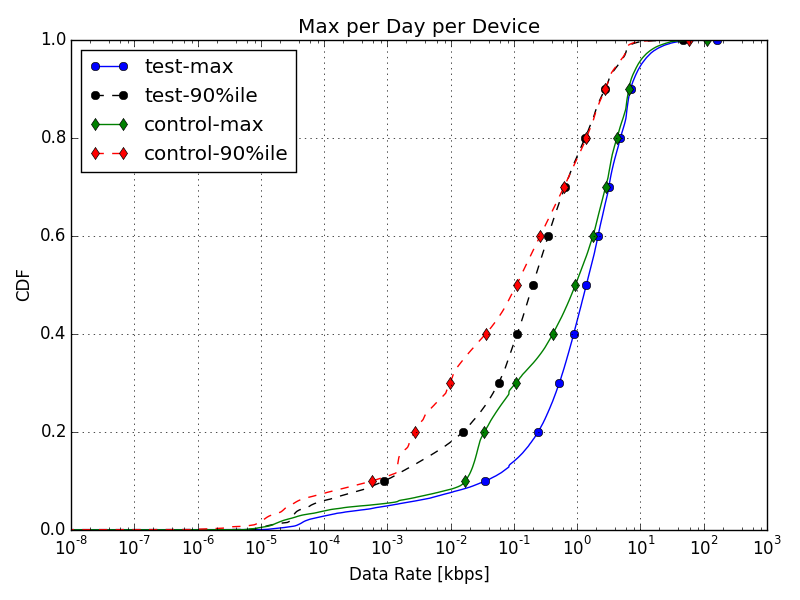
\includegraphics[width=\linewidth]{figures/cdf-max-per-day-per-device.png}
  \caption{CDF of max per device daily}
  \vspace{1em}
  
%http://sites.noise.gatech.edu/~sarthak/files/comcast/plots/full_dw/cdf-max-per-
%day-per-device.png
  \label{fig:CDF-data-rate-max-daily}
\end{subfigure}
%\hfill
\end{minipage}
\caption{Peak Utilization: The maximum data rate varies for test and control 
set 
for low data rates, and this variation is present daily.}
\label{fig:peak-utilization}
% created using docs/metadata-separated.log
\end{figure}



Based on the measurement methodology, we study the highest utilization seen by a 
household
both in its lifetime, and on each day. Our aim is to examine the peak usage per 
household, and
study if the behavior changes due to an upgrade.

Figure~\ref{fig:CDF-data-rate-max} provides a distribution of the highest 
average
data rate a household achieves. To avoid outliers, we also plot the 90\%-ile of 
the max
data rate achieved by households in both \test and \control sets. We see that a 
median
household is expected to achieve the highest data rate of between 1 -- 10 Mbps 
over its
lifetime. This is much lower than the access link capacity,
indicating that the median device has a utilization ratio (avg data 
rate:capacity) under
0.1 in our dataset. The number of households that increased their peak 
utilization beyond
the \control set's 105 Mbps capacity were negligible.

Surprisingly, we see that 30\% of the households from the \test set have a low 
peak
utilization (under 0.1 Mbps), while 40\% of the \control set households are 
under 0.1 Mbps.
Thus, the absolute peak utilization does not increase when compared to the 
access link
capacity, but there is certainly an increase in peak utilization of devices that 
had a low
requirement, due to the change in capacity.

To investigate this further, we also study the \emph{peak utilization per device 
on a daily basis}.
Figure~\ref{fig:CDF-data-rate-max-daily} shows that for 30\% of the devices,
the maximum data rate in the \test set is consistently higher than the \control 
set, albeit
no where near the actual access link capacity.

This is similar to the behavior observed in figure~\ref{fig:TS-data-rate-daily}, 
showing that the peak
usage during prime-time is unaffected, but lower utilization throughout the day 
is higher
for the test set. We speculate that there could be two possible reasons for this 
increase
in utilization: (1) short term downloads and/or web browsing achieves a slightly 
better
data rate on a small time scale, or (2) real-time video quality is slightly 
higher, but
not enough to completely saturate the access link capacity. Unfortunately, we 
miss these
short lived, or consistent, events due to a 15 minute time slot granularity and 
only
looking at byte counters.



\paragraph{Peak Ratio: }The Sandvine Reports show that although the mean usage has remained
stable for the past few years, usage during peak-times has increased
drastically~\cite{sandvine20141h}. To measure this growth, they introduce the
concept of peak period, measured when the network is within 95\% of its highest point.
Although, these reports present a good view into aggregate usage patterns over a month,
they neglect to analyze usage characteristics individually. Inspired by their
definition, we measure the disparity between the 90 percentile of the peak and median
usage of each household within a day, and call this the \emph{Peak-Ratio}. In
section~\ref{subsec:peakratio} we show that the peak ratio can be used
to divide users in the same tier based on their usage behavior.

% the ratio of the 90\%-ile to the median throughput per day.


\begin{figure}[ht]
\begin{minipage}{0.90\linewidth}
\centering
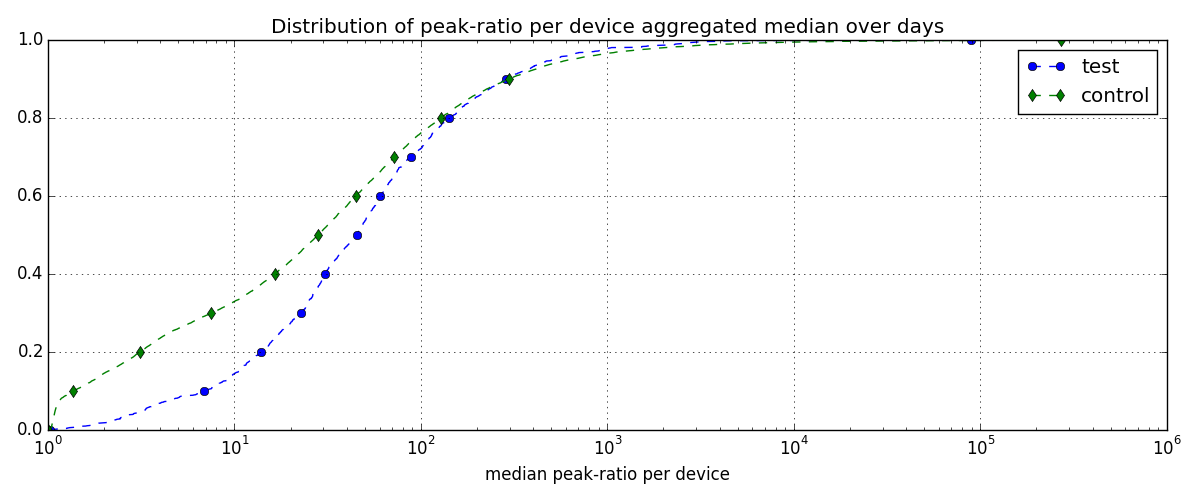
\includegraphics[width=1\linewidth]{figures/peakratio-CDF-devices-MEDIAN.png}
\caption{Median peak ratio per device showing that test set has higher daily ratio (50 times by median). Thus ISPs should condition their networks to 50 times the median usage for each user added in the worst case scenario.}
%http://sites.noise.gatech.edu/~sarthak/files/comcast/plots/full_dw/peakratio-CDF-devices-MEDIAN.png
\label{fig:CDF-peak-ratio-median}
\end{minipage}
\end{figure}

To further characterize and compare the deviation of data rate for the \control and \test set, we examine \emph{peak-ratio} as defined above. 
Figure ~\ref{fig:CDF-peak-ratio-median} shows that the median peak-ratio for each device in the \test set is much larger than that of the \control set.
\todo{replace much larger with the exact number or percentage}.
\sg{Taken together} with our observations of a lower prime-time ratio of the \test set (section~\ref{subsec:primetime}) this implies that there are households in the \test set that achieve a peak-ratio $>$ 1, but not during the prime-time hour. We believe that these households might actually be small businesses or work-at-home users that peak during daytime hours instead of evening hours.

\begin{figure}[ht]
\begin{minipage}{0.9\linewidth}
\centering
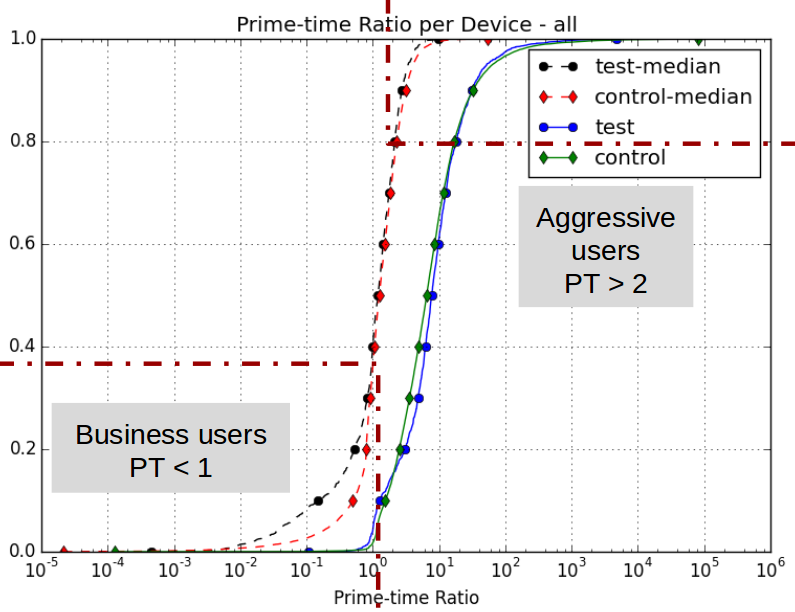
\includegraphics[width=0.9\linewidth]{figures/cdf-prime-time-ratio[replace].png}
\caption{(old) Prime Time ratio + usage can be used to divide users into four sets: aggressive all time + non aggressive all time, aggressive peak time, aggressive non-peak time (business hours). 30\% PT $<$ 1: possibly businesses with normal work-hours . 20\% PT $>$ 2: aggressive prime-time streamers}
%http://riverside.noise.gatech.edu:8083/separated/full/cdf-prime-time-ratio-per-device.png\\
%http://riverside.noise.gatech.edu:8083/plots/full_dw/prime-time-ratio-per-device-cdf-ALL.png
\label{fig:CDF-prime-time-ratio}
\end{minipage}
\end{figure}

The median peak-ratio per device itself shows a large range, from 1 to 10e6 (figure~\ref{fig:CDF-peak-ratio-median}), and the maximum peak-ratio per device was an order higher. Clearly there are some households that have a very even usage throughout the day (low peak ratio), and others that are extremely aggressive only at certain times (high peak ratio). We plot this segregation in figure ~\ref{fig:CDF-prime-time-ratio}.


% other results:
%big difference (2 x median ratio) in per device per day ratios of 90%ile:median.
%weird shape again for values < ratio 100
%big difference in this ratio per day, and it is consistent across all individual sets + months.
%very large for Dec, slightly smaller for Nov
%interestingly, at higher ratios control is slightly > test. This means that certain devices in control set have a huge std (ratio) in a day as compared to test set which has a lower “max” ratio.

\todo{ TO PLOT? :}
\begin{itemize}
\itemsep0em
\item peak ratio cdf vs no of devices
\item peak ratio cdf vs time of day where peak occurred
\item no of devices cdf vs time of day where peak occurred
\end{itemize}

Based on differing usage profiles within the same high tier bandwidth, we suggest that the FCC adopt multiple benchmarks based on usage characteristics to better characterize broadband availability, deployment, and adoption in the US. Such multiple benchmarks can be the minimum broadband speed required per user based on the kind of traffic expected during a day. ISPs can also offer these users better plans based on hour-of-the-day or usage caps to encourage more off-peak usage. These users probably don't cause latency spikes in PT.